80. $g(x)=\cfrac{2x+1}{2x^2+x}=\cfrac{2x+1}{x(2x+1)}=\cfrac{1}{x},\ x
eq-\cfrac{1}{2}.$
$$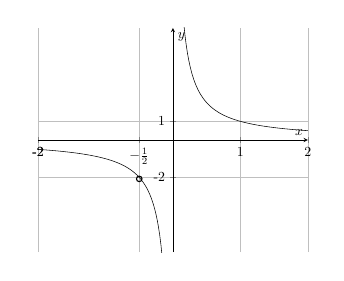
\begin{tikzpicture}[scale=0.5]
\begin{axis}[
    axis lines = middle,
    grid=major,
    legend pos={south west},
    xlabel = {$x$},
    %xlabel style={below right},
    ylabel = {$y$},
    ymin=-6,
    ymax=6,
    xmin=-2,
    xmax=2,
    xtick={-2, -2, -0.5, 1, 2},
    xticklabels={-2, -2, $-\frac{1}{2}$, 1, 2},
    ytick={-2,1},
    yticklabels={-2,1},
                  ]
	\addplot[domain=-2:-0.1, samples=100, color=black] {1/x};
    \addplot[domain=0.1:2, samples=100, color=black] {1/x};
        %\addplot[domain=2.01:6, samples=100, color=black] {2/(2-x)};
   % \addplot[domain=-3:3, samples=100, color=black] {-x};
     %\addlegendentry{$\text{Рис. 1}$};
\end{axis}
\draw (2.57,1.86) circle (2pt);
%\draw (3.45,0.75) circle (2pt);
%\draw (3.45,2.55) circle (2pt);
\end{tikzpicture}$$
а) Прямая $y=kx$ имеет с графиком $g(x)$ одну общую точку, если проходит через точку $\left(-\cfrac{1}{2};-2
ight),$ то есть если $-\cfrac{1}{2}k=-2,\ k=4.$\\
б) Для нахождения общих точек графика и прямой, составим уравнение $\cfrac{1}{x}=bx+2,\ bx^2+2x-1=0,$ при этом $x
eq-\cfrac{1}{2}.$ Это уравнение имеет один корень либо при $b=0$ $\left(\text{тогда }x=\cfrac{1}{2}
ight),$ либо при $\cfrac{D}{4}=1+b=0,\ b=-1\ \left(\text{тогда }x=1
ight),$ либо если одним из корней является $x=-\cfrac{1}{2},$ то есть $b\cdot\cfrac{1}{4}-1-1=0,\ b=8.$\\
